\chapter{Diskussion}

In Kapitel \ref{sec:snp_auswertung} wurde gezeigt, dass \ac{SNP}s sich in Unterschieden in \ac{EP} ausdrücken. Nun soll diskutiert werden in wie fern sich \ac{SNP}s mittels \ac{EP}s annotieren lassen können.

\section{SNPs in Energieprofilen}
\label{sec:snps_in_eps}

\begin{figure}
    \centering
    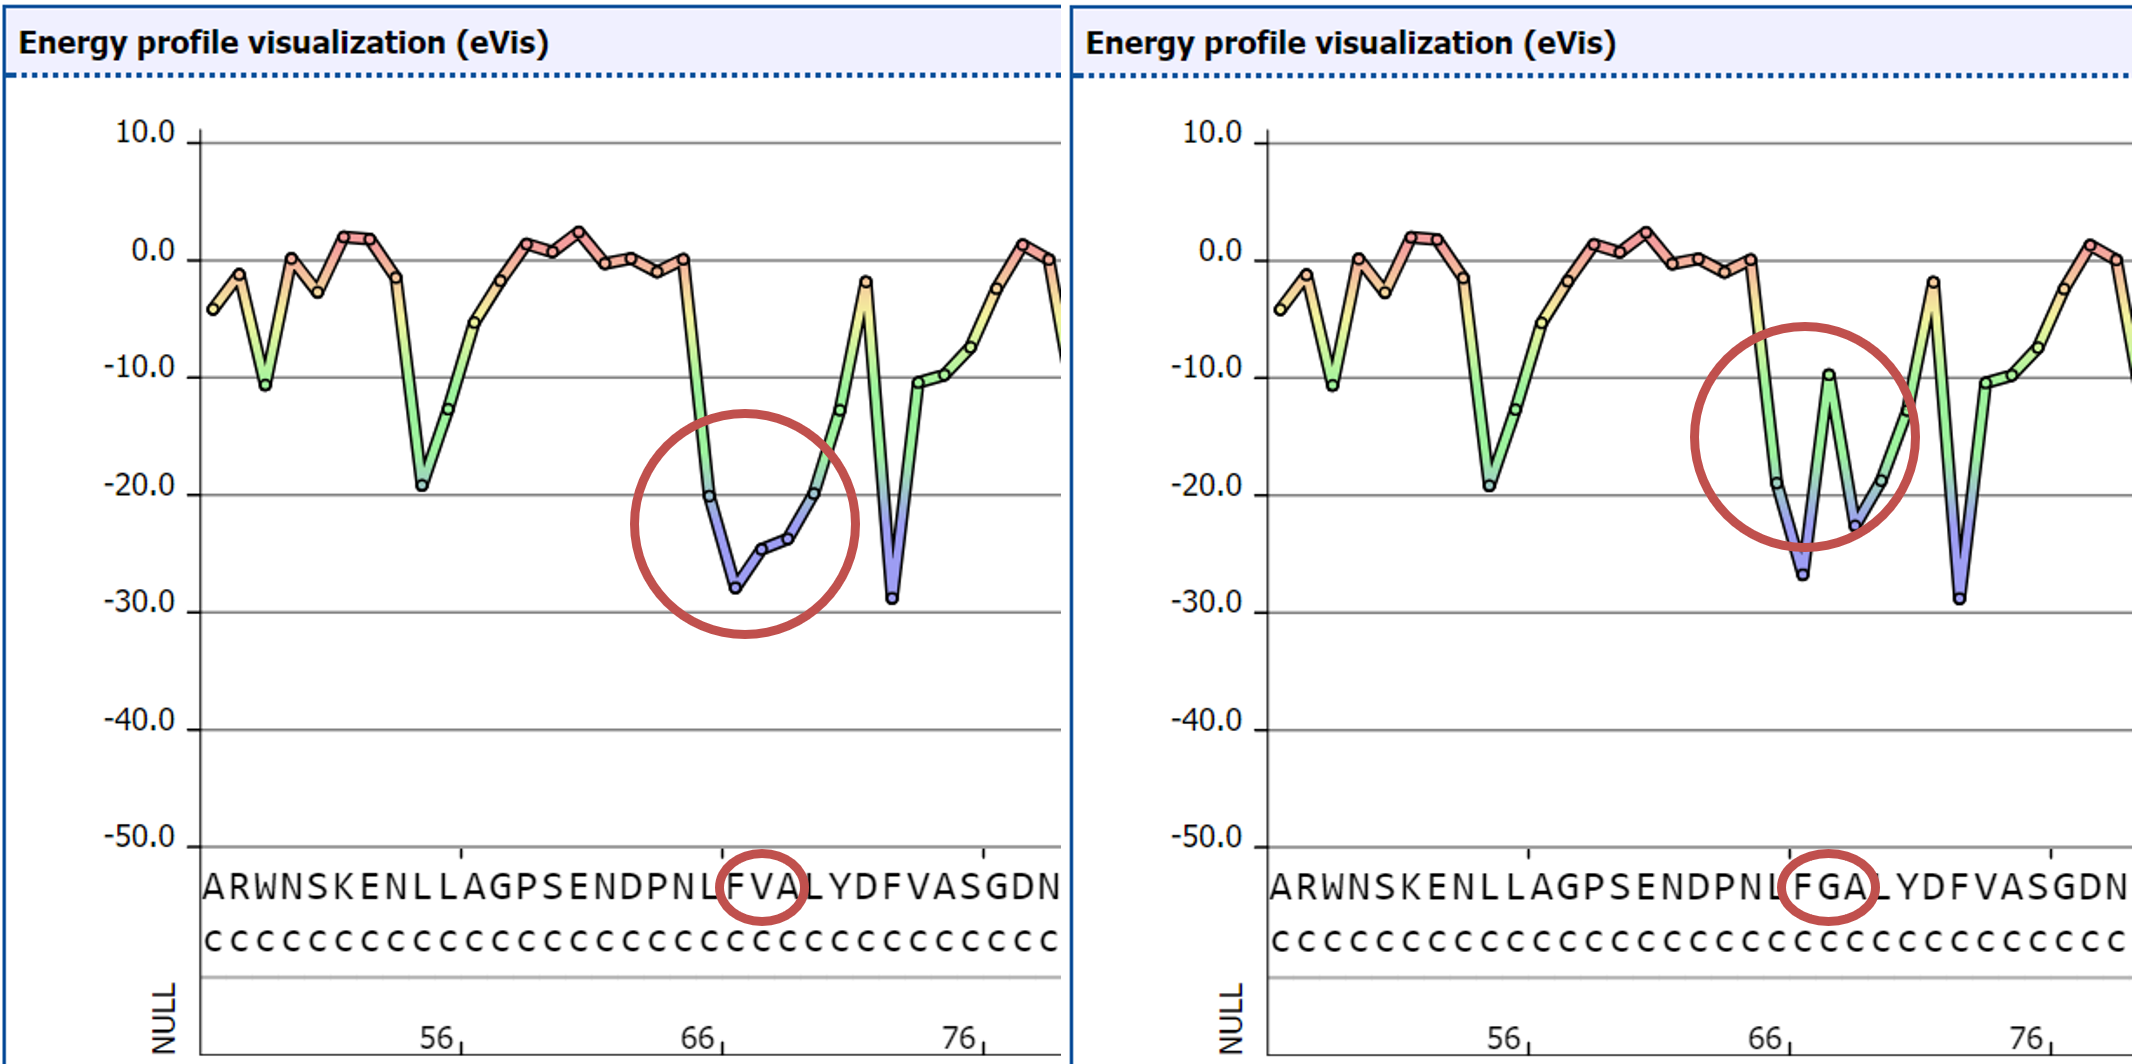
\includegraphics[width=.99\textwidth]{images/ep_vs_snp.png}
    \caption{\ac{eVis} Darstellung vom ePros Webserver (Kapitel \ref{sec:epros}) eines Ausschnittes eines \ac{EP}s. Die original Sequenz befindet sich links und Sequenz mit dem \ac{SNP}(rote Markierung) ist rechts. Auf der Abszisse sind die Aminosäuren im Einbuchstabencode aufgetragen, siehe Tabelle \ref{tab:amino_table}. Darunter ist die Sekundärstruktur als Buchstabencode und visualisiert aufgetragen. Unten ist die Aminosäureposition in 10er Schritten aufgetragen. Auf der Ordinate befinden sich die Energiewerte.}
    \label{fig:ep_vs_snp}
\end{figure}

Bei dem Vergleich von \ac{EP}s mit \ac{SNP} gegen das unmutierte \ac{EP} ist aufgefallen, dass sich die \ac{EP}s signifikant an den \ac{SNP} Positionen unterscheiden. Zum Verständnis ist ein \ac{EP} (mit und ohne \ac{SNP}) in \ac{Abb} \ref{fig:ep_vs_snp} dargestellt. Hier sieht man eine 2D Visualisierung eines \ac{EP}s, auf der Abszisse sind die Aminosäuren im Einbuchstabencode aufgetragen, wahrend auf der Ordinate die Energiewerte eingetragen sind. Die beiden Darstellungen unterscheiden sich nur durch die Substitution von Valin durch Glycin, so ist hier deutlich die Energiewert Differenz zwischen den beiden Darstellungen zu erkennen. So besitzt im Protein Valin an der Position 68 einen Energiewert von -25, der Glycin \ac{SNP} hingegen besitzt einen Energiewert von -10, so ergibt sich eine Delta von 15. 

Valin ist eine hydrophobe Aminosäure, während Glycin eine hydrophile Aminosäure ist, von daher ist es nicht überraschend, dass sich auch die Energiewerte des Proteins an dieser Stelle bei einem Austausch verändern. Dies zeigt uns deutlich, dass wir drastische Veränderungen der Proteinstruktur auch in den \ac{EP}s sehen.

Sieht man sich nun mit diesem Wissen \ac{Abb} \ref{fig:comp_plot_MSH2} an, so sieht man das der gutartige \ac{SNP} das \ac{EP} fast gar nicht verändert. Dies wird auch bestätigt, wenn man sich die chemischen Eigenschaften von Valin anschaut, denn Valin ist unpolar, genauso wie das Isoleucin welches es ersetzt hat. Zudem haben beide Aminosäuren in etwa die gleiche Größe. 

Generell sieht man das das \ac{EP} sich fast gar nicht verändert und die gesamte Energiedifferenz bei gerade mal -0,006 liegt. Dies passt alles sehr gut zu der ClinVar annotation, welche sagt das dieser \ac{SNP} gutartig ist.

Betrachten wir nun die untere \ac{Abb} in \ref{fig:comp_plot_MSH2}, so sehen wir, dass sich die Energie sich stark am \ac{SNP} verändert. Auch generell sieht man das sich die Energie im gesamten Protein viel stärker als im gutartigen \ac{SNP} in der oberen \ac{Abb} verändert. Wenn man sich die chemischen Eigenschaften von Glycin ansieht, sieht man das es polar ist, bei Tryptophan hingegen handelt es sich um eine unpolare Aminosäure. Zusätzlich ist Glycin die kleinste Aminosäure, während Tryptophan wesentlich größer ist. Auch dies passt gut zur ClinVar Annotation, welche besagt, dass es sich hierbei um ein pathogenes \ac{SNP} handelt.

Sehr ähnlich Verhält es sich mit der \ac{Abb} \ref{fig:comp_plot_ACADM}, hier ist im oben Bild ein gutartiges \ac{SNP} des Gens \texttt{ACADM} dargestellt. Hier sieht man wie in \ac{Abb} \ref{fig:comp_plot_MSH2} nur eine kleine Veränderung der Energie. Bei Methionin handelt es sich um eine hydrophobe Aminosäure genau wie bei Isoleucin, so scheint dieser \ac{SNP} chemisch keine große Veränderung zu machen. Diese Annahme wird auch von der ClinVar Annotation gutartig bestätigt. 

Sieht man sich hingegen das untere Bild an, so fällt eine sehr starke Veränderung des Energieniveaus am \ac{SNP} auf. Nach bisherigem wissen würden wir diesen \ac{SNP} also als pathogen einordnen, dies ist richtig, wenn man die ClinVar Annotation hinzuzieht. Auch die chemischen Eigenschaften der Threonin unterscheiden sich von den der Aminosäure Isoleucin, denn Threonin ist polar und Isoleucin nicht. 



\section{Anwendbarkeit der EPs zur Annotation von SNPs im Panel}

In Kapitel \ref{sec:snps_in_eps} wurde gezeigt, dass es möglich ist Energieprofile zu nutzen um \ac{SNP}s zu annotieren.  Die Auswertung der \ac{SNP}s aus Tabelle \ref{tab:snps_memb} und \ref{tab:snps_glob} ergab, dass dies Möglich ist und ein MCC von 0,8 für globuläre und sogar 1,0 für Membran assozierte Proteine erreicht werden kann. Doch jetzt stellt sich die Frage, ob wir die Erkenntnisse der Arbeit nutzen können um die im Illumina TruSight Myeloid Sequencing Panel auftretenden Gene zu annotieren. 

Dafür wurde zuerst versucht per Hand die einzelnen Gen Sequenzen herunterzuladen und anschließend in Swissmodel zu modellieren. Doch leider lieferte dies nicht die gewünschten Ergebnisse, die Coverage war in den meisten Fällen sehr schlecht. So bewegte sich z.B. die Coverage für \texttt{NRAS} zwischen 1-4\%, sodass nur einzelne Helices abgedeckt waren. Dieses Bild zeigte sich so, oder so ähnlich für alle getesteten Proteine. 

\begin{table}[]
    \centering
    \caption{Illumina TruSight Myeloid Sequencing Panel Gene \emph{coverage}, Transkriptlänge ist mit UTRs und CDS angegeben.}
    \label{tab:illumina_coverage}
    \resizebox{\linewidth}{!}{%
    \begin{tabular}{lllll}
    \hline
    \multicolumn{1}{|l|}{Genname} & \multicolumn{1}{l|}{Genlänge (bp)} & \multicolumn{1}{l|}{Transkriptlänge} & \multicolumn{1}{l|}{PDB-ENSP} & \multicolumn{1}{l|}{PDB Coverage} \\ \hline
    IDH1 & 29847 & 2298 & 1t09.A & 17,97\% \\
    KDM6A & 239425 & 5438 & 3avr.A & 9,58\% \\
    JAK2 & 143793 & 5285 & 4z32.A & 9,18\% \\
    NRAS & 12425 & 4449 & 3con.A & 3,84\% \\
    RAD21 & 28931 & 3749 & 4pju.B & 3,71\% \\
    NOTCH1 & 51418 & 9371 & 3eto.A & 3,06\% \\
    \end{tabular}}
\end{table}

Aus diesem Grund wurde der EnsemblBioMart\footnote{\url{https://www.ensembl.org/biomart}} hinzugezogen, dieser ermöglicht es dem Nutzer leicht spezielle Datensätze mit verschiedensten Filtern herunter zu laden. So wurde in diesem Fall die Genliste des Illumina Panels mit 54 Genen im BioMart eingefügt und Genlänge, Transkriptlänge, korrespondierende \ac{PDB} Einträge und deren Start und Stopp Position abgefragt, dargestellt in Tabelle \ref{tab:illumina_coverage}. Die Start und Stopp Position der \ac{PDB} Einträge wurde mit der Transkriptlänge verrechnet, so dass eine prozentuale Coverage abgebildet werden kann. Wie zu sehen ist, besitzt \texttt{IDH1} die beste Coverage mit 17,97\%, dies ist leider viel zu wenig um eine erfolgreiche Berechnung eines \ac{EP}s durchzuführen. Bei den anderen Genen sieht es leider noch schlechter aus, denn von den 54 Genen im Panel weisen gerade mal 6 Gene überhaupt eine Teilabdeckung auf. 

\begin{table}[]
    \centering
    \caption{VariantPlex Solid Tumor Kit Coverage, Transkriptlänge ist mit UTRs und CDS angegeben.}
    \label{tab:variantplex_coverage}
    \resizebox{\linewidth}{!}{%
    \begin{tabular}{lllll}
    \hline
    \multicolumn{1}{|l|}{Genname} & \multicolumn{1}{l|}{Genlänge (bp)} & \multicolumn{1}{l|}{Transkriptlänge} & \multicolumn{1}{l|}{PDB-ENSP} & \multicolumn{1}{l|}{Coverage} \\ \hline
    ATM & 146618 & 12954 & 5np0.A & 23,58\% \\
    IDH1 & 29847 & 2298 & 1t09.A & 17,97\% \\
    H3F3A & 10150 & 799 & 3av2.A & 16,90\% \\
    RB1 & 178235 & 4840 & 4elj.A & 15,17\% \\
    BRAF & 205437 & 2480 & 4mnf.A & 12,26\% \\
    PIK3CA & 91979 & 9093 & 2rd0.A & 11,73\% \\
    SMO & 24673 & 3738 & 5v56.A & 10,27\% \\
    RHOA & 53853 & 2031 & 1ftn.A & 9,45\% \\
    JAK2 & 143793 & 5285 & 4z32.A & 9,18\% \\
    CCND1 & 13387 & 4307 & 2w96.A & 6,27\% \\
    ALK & 728792 & 6220 & 4fob.A & 5,66\% \\
    DDR2 & 156027 & 3096 & 2wuh.A & 5,43\% \\
    ROS1 & 137555 & 7435 & 3zbf.A & 4,01\% \\
    SMAD4 & 56651 & 8495 & 1dd1.A & 3,14\% \\
    NOTCH1 & 51418 & 9371 & 3eto.A & 3,06\% \\
    MYCN & 6443 & 2602 & 5g1x.B & 2,34\%
    \end{tabular}}
\end{table}

Um zu überprüfen, ob es sich bei dem Illumina Panel nicht um eine unglückliche Ausnahme handelt wurde noch ein zweites Panel überprüft. Das \emph{VariantPlex Solid Tumor Kit}\footnote{\url{http://archerdx.com/variantplex/solid-tumor}} umfasst 67 Gene im Zusammenhang mit soliden Tumoren. Doch auch hier ist nur ein Bruchteil der Gene aufgeklärt und von diesen 16 Genen, ist keines komplett strukturell aufgeklärt. Die höchste Coverage hat \texttt{ATM} mit 23,58\%, dies ist jedoch immer noch zu wenig um damit eine Homologie Modellierung durchzuführen. Auch dieses Panel beinhaltet \texttt{IDH1} und weist damit ebenfalls eine Coverage von 17,97\% auf gefolgt von \texttt{H3F3A} mit einer Coverage von 16,90\%. Bei den restlichen Treffern fällt die Coverage stark ab.

Somit lässt sich abschließend sagen, dass sich \ac{APs} (noch) nicht für die Annotation von \ac{SNP}s im Illumina TruSight Myeloid Sequencing Panel eignen, da einfach noch zu wenige Strukturen aufgeklärt sind. Denn ohne aufgeklärte Struktur macht es keinen Sinn ein Homologie Berechnung durchzuführen, denn wie in \ref{sec:min_coverage} gezeigt, würde das Ergebnis unbrauchbar sein. Sodass keine \ac{EP} Berechnung durchgeführt werden kann. 


\subsection{Minimale Coverage und Sequenzidentität}
\label{sec:min_coverage}

In diesem Abschnitt wird diskutiert, welche minimale Coverge ein Proteine haben muss damit es Sinn macht ein \ac{EP} dafür zu berechnen. Denn es hat sich herausgestellt das die Vorhersage eines \ac{SNP}s sehr stark abhängig von dem Template ist.

\begin{figure}
    \centering
    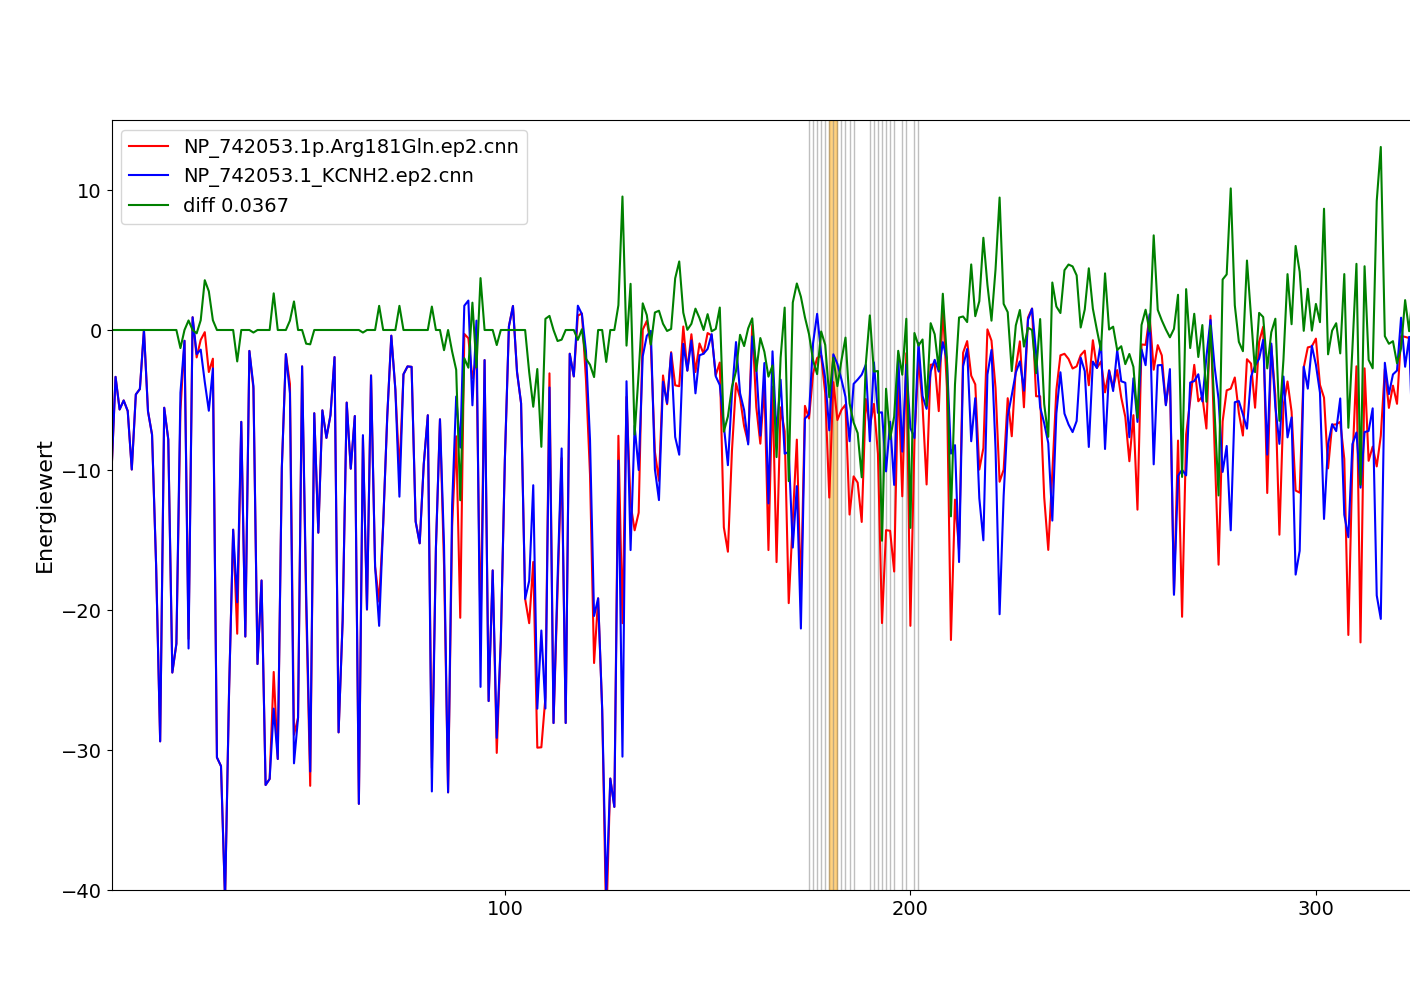
\includegraphics[width=.99\textwidth]{images/comp_plot_KCNH2_Arg181Gln.png}
    \caption{Fehlerhafter Plot, eigentlich benign ist aber jenseits von gut und böse}
    \label{fig:fail_ep}
\end{figure}


%- Überprüfen ob Sequenz identität wichtig ist? 



\subsection{Problem mit dem Datensatz}
- Warum ist keien perfekte Trennung der SNPs möglich?

- Fehler im Modell

- Gesamter Ansatz
- ClinVar hat nicht die Warheit

- Mutations an sich ist nicht benign
- Fehlende zusatzdaten -> wird aufgehoben ?
- Patienten alter, und co

- Problem zu wenige benign SNPs
- 


Entweder Protein vollständig aufgeklärt, wie \url{ABCG2} \url{https://www.ncbi.nlm.nih.gov/pubmed/?term=28554189} oder \texttt{KCNH2} \url{http://www.rcsb.org/pdb/explore/explore.do?structureId=5VA1} aber dafür keine mehrfach bestätigten SNPs, oder viele mehrfachbestätige SNPs, jedoch keine vollständige 3D Struktur, siehe...

SNPs liegen nicht in der aufgeklärten 3S Struktur, siehe ...

SNPs liegen auf verschiedenen Transkripten ...

Sequenz Identität ist nicht ausreichend, siehe ...

Noch nicht ausreichend 3D Strukturen:

Die Anzahl aufgeklärter 3D Strukturen liegt bei XX\% bei einem Wachstum von XX, hingegen die 3D Strukturen nur XX\% bei einem Wachstum von XX\%. Sodass es im Jahr XXYY XY\% zu erwarten sind * Quelle: "Trends in structural coverage of the protein universe and the impact of the Protein Structure Initiative"


UniProtKB/Swiss-Prot enthält seit dem 22. Juli 2008 etwa 400K-Sequenzeinträge, während die Protein-Datenbank (PDB) nur etwas mehr als 50K experimentell bestimmte Proteinstrukturen enthält. 
Quelle (An integrated database for complex protein structure modeling) Aus <http://ieeexplore.ieee.org/document/4686206/?reload=true> 
Heute:  
555.426 sequence entries Aus \url{http://web.expasy.org/docs/relnotes/relstat.html} 
133.589 Biological Macromolecular Structures aus \url{https://www.rcsb.org/pdb/statistics/contentGrowthChart.do?content=total&seqid=100}

Wobei nur einige PDB Einträge nur Subdomänen von Proteinen sind
Ein PDB Eintrag =/= Eine komplette Squenz

Das gilt für alle Strukturen über alle Spezies, für den Homo Sapiens gibt es also nur ein Teilsatz an 3D Strukturen.
    >Wie viele Gene hat der Mensch? >
    "29 000. Die ungefähre Lokalisation von 22 000 Genen ist bereits bekannt."
Aus \url{https://www.deutsche-apotheker-zeitung.de/daz-az/2001/daz-11-2001/uid-389}

"Each of the estimated 30,000 genes in the human genome makes an average of three proteins."
Aus \url{https://www.genome.gov/11006943/human-genome-project-completion-frequently-asked-questions/}







%\section{Ramachandran Diskussion}

%Winkelveränderung
%- In der Mutation
%- In den Kontakten




zusätzliches

nicht alle Aminosäuren im gleichen Energiespektrum zu finden sind.